\renewcommand{\vec}[1]{\mathbf{#1}}
\newcommand{\N}[1]{\mathcal{N}\left(#1\right)}
\newcommand*{\T}{^{\mkern-1.5mu\mathsf{T}}}
\newcommand{\ud}[1]{\underline{\smash{#1}}}

\frame{\frametitle{Introduction}
\begin{itemize}
  \item You've all probably heard of them.
  \item It's a hot topic in data science, along with neural nets and machine
    learning.
  \item You might have heard that they provide a non-parametric function model.
  \begin{itemize}
    \item Or just that they depend on hyperparameters.
  \end{itemize}
  \item Or that they can fit an arbitrery function.
  \item Or seen figures like these:
\end{itemize}
}

\begin{frame}[plain]
  \vspace{-5mm}
  Google image search for ``Gaussian process" \\
  {\color{white}\rule{2mm}{5mm}}
  \hspace*{-6.3mm}
  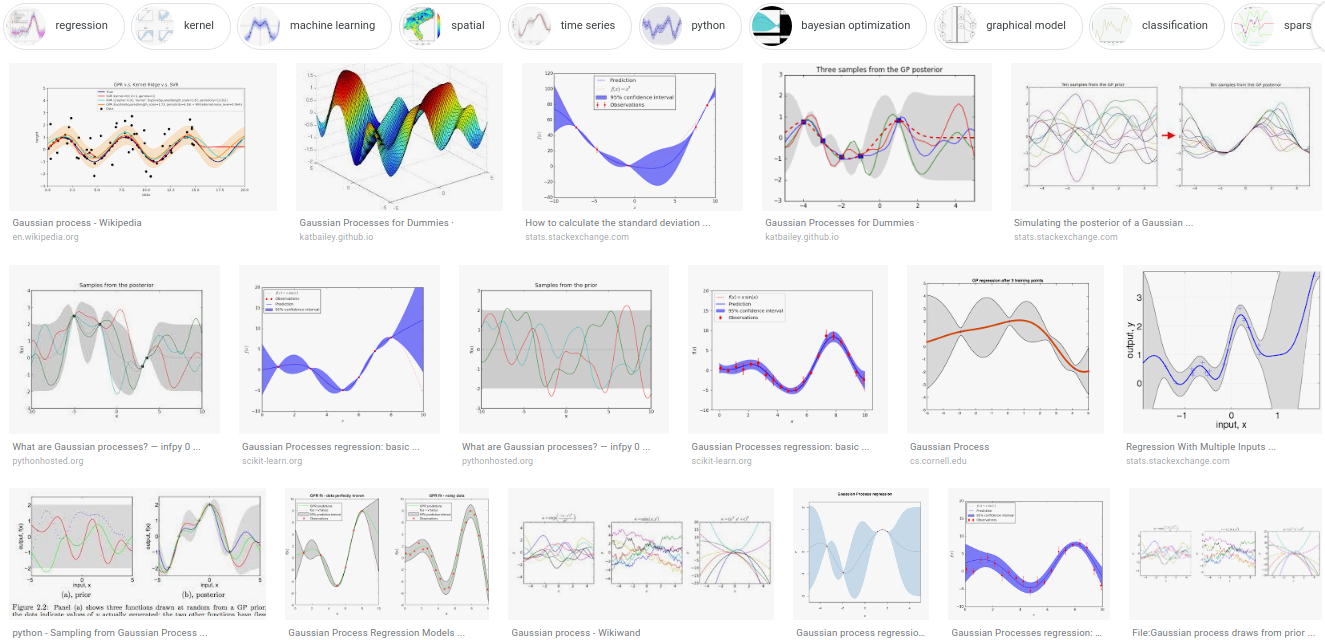
\includegraphics[width=\paperwidth]{google}
\end{frame}

\frame{\frametitle{Definition}
\begin{itemize}
  \item One of the most commonly seen defenitions of a GP is this:
\end{itemize}
\begin{tcolorbox}
  A Gaussian process is a collection of random variables, any finite number
  of which have a joint Gaussian distribution.
\end{tcolorbox}
\begin{itemize}
  % I hate it, because it provides no intuition about the usefulness of the
  % mathematical object or the inference method that utilizes it.
  \item This is like saying that a fork is something that splits at one end. \\
  An accurate, yet uninspiring statement.

  \vspace{5mm}
  \item We'll return to the definition later.
\end{itemize}
}

\begin{frame} \frametitle{The first step}
\begin{itemize}
  \item Assume we made an observation of a vector
    $\vec{d} = [y_1,y_2,\mathellipsis,y_n]$,\\
    and that $\vec{d}$ is sampled from a multivariate Gaussian
    distribution,\\i.e. $\vec{d}\sim\N{\vec{0},D}$.
  \vspace{1mm}
  \item Assuming non-zero mean is no more general, because the mean can be
    absorbed into the defenition of $\vec{d}$.
  \vspace{1mm}
  \item If we arbitrarily split $\vec{d}$ into subvectors
    $\vec{a}$ and $\vec{b}$, then we can write
\end{itemize}
\begin{equation}\label{eq:n1}
  \begin{bmatrix} \vec{a} \\ \vec{b} \end{bmatrix} \sim
    \N{\vec{0},\begin{bmatrix} A & C \\ C\T\!\! & B \end{bmatrix}}
\end{equation}
\begin{itemize}
  \item The conditional probability of $\vec{b}$ given $\vec{a}$ is
\end{itemize}
\vspace{1mm}
\begin{equation}
  p(\vec{b}|\vec{a})
  = \frac{p(\vec{a}\cap\vec{b})}{p(\vec{a})}
  = \frac{p(\vec{d})}{\int p(\vec{d})p(\vec{b}') \mathrm{d}\vec{b}'}
  = \boxed{ \N{C\T\!A^{-1}\vec{a},\,B-C\T\!A^{-1}C} }
\end{equation}
\vspace{-5mm}
\begin{itemize}
  \item Proof: {\small\url{https://stats.stackexchange.com/q/30588/239215}}
\end{itemize}
\end{frame}

\begin{frame} \frametitle{Bayesian Inference}
\vspace{-2mm}
\begin{itemize}
  \item Recall the Bayes' theorem
\end{itemize}
\vspace{1mm}
\begin{equation}
  \text{posterior} =
  \frac{\text{likelihood}\times\text{prior}}{\text{marginal likelihood}},
  \quad
  p(\vec{b}|\vec{a}) = \frac{p(\vec{a}|\vec{b})}{p(\vec{a})}\,p(\vec{b}).
\end{equation}
\begin{itemize}
  \item $p(\vec{b}) = \N{\vec{0},B}$ can be viewed as the \ud{prior},
    and $p(\vec{b}|\vec{a}) = \N{C\T\!A^{-1}\vec{a},\,B-C\T\!A^{-1}C}$ as the
    \ud{posterior}. \\
    {\small\color{gray} * Conditioning}
  \vspace{1mm}
  \item GP is defined by the multivariate Gaussian distribution in
    Eq.~\ref{eq:n1}.
  \vspace{1mm}
  \item Clearly, we didn't have to have observed the $\vec{b}$ part of the
    vector to make this inference.
  \vspace{1mm}
  \item In GP regression, inference is made about unobserved function values.
  \begin{itemize}
    \item Think of a function as a (generally continuous infinite-dimensional)
      vector, whose elements are labeled by the coordinates on the manifold
      on which the function lives.
  \end{itemize}
  \vspace{1mm}
  \item Non-zero convariance, $C$, contains the additional information. \\
    Otherwise, $p(\vec{b}) = p(\vec{b}|\vec{a})$.
\end{itemize}
\end{frame}

\begin{frame} \frametitle{GP Regression}
\begin{itemize}
  \item Given: observed function values, $y_i$, at points $x_i$.
  \item Model: prior distribution of the function values,
    given my the mean $m$ and covariance matrix $K$.
    This is the GP.
\end{itemize}
\begin{equation}
  f(x) \sim \N{m(x),K(x,x')}
\end{equation}
  \vspace{-7mm}
\begin{itemize}
  \item Take $m = 0$ for brevity
  \item For observed values $y$, and unobserved values $y_*$, we can
    write
\end{itemize}
\begin{equation}
  \begin{bmatrix} y \\ y_* \end{bmatrix} \sim
  \N{0,\,\begin{bmatrix} K(x,x) & K(x,x_*) \\ K(x_*,x) & K(x_*,x_*) \end{bmatrix}},
  \ \text{or}
\end{equation}
\begin{equation}
  \begin{bmatrix} y \\ y_* \end{bmatrix} \sim
    \N{0,\,\begin{bmatrix} K & K_* \\ K_*\T\!\! & K_{**} \end{bmatrix}}.
\end{equation}
  \vspace{-4mm}
\begin{itemize}
  \item Then,
\end{itemize}
\begin{equation}
  \boxed{ y_*|y \sim \N{K_*\T K^{-1}y,\,K_{**}-K_*\T K^{-1}K_*} }
\end{equation}
\end{frame}

\begin{frame} \frametitle{GP Regression}
\begin{equation}
  \boxed{ y_*|y \sim \N{K_*\T K^{-1}y,\,K_{**}-K_*\T K^{-1}K_*} }
\end{equation}
\begin{itemize}
  \item Gives the best linear unbiased prediction.
  \item Direct measure of uncertainty at each point of the function.
  \item Function value predictions are independent.
  \begin{itemize}
    \item Can compute point-by-point. \hspace{5mm}
    {\small\color{gray} * Lazy learning}
  \end{itemize}
  \item Also called Kriging.
  \begin{itemize}
    \item The theoretical basis for the method was developed by the French
      mathematician Georges Matheron in 1960, based on the Master's thesis of
      Danie G. Krige, the pioneering plotter of distance-weighted average gold
      grades at the Witwatersrand reef complex in South Africa.
      [\href{https://en.wikipedia.org/wiki/Kriging}{Wikipedia}]
  \end{itemize}
\end{itemize}
\end{frame}

\begin{frame} \frametitle{GP Regression Algorithm}
\begin{equation}
  \boxed{ y_*|y \sim \N{K_*\T K^{-1}y,\,K_{**}-K_*\T K^{-1}K_*} }
\end{equation}
\begin{equation}
  \bar{y}_* = \vec{k}_*\T K^{-1} \vec{y}, \quad
  \mathrm{var}(y_*) = k_{**} - \vec{k}_*\T K^{-1} \vec{k}_*
\end{equation}
\vspace{-3mm}
\begin{itemize}
  \item In practice, instead of inverting the $K$ matrix, \\
    Cholesky decomposition is used: $K = LL\T$.
  \begin{itemize}
    \item $K$ is symmetric.
    \item $L$ is triangular.
  \end{itemize}
  \vspace{1mm}
  \item Then $K^{-1} = (L^{-1})\T L^{-1}$, so
\end{itemize}
\begin{equation}
  \bar{y}_* = \left(L^{-1}\vec{k}_*\right)\T \left(L^{-1} \vec{y}\right),
  \quad
  \mathrm{var}(y_*) = k_{**} -
    \left(L^{-1}\vec{k}_*\right)\T
    \left(L^{-1}\vec{k}_*\right)
\end{equation}
\vspace{-5mm}
\begin{itemize}
  \item Cholesky decomposition \plus\ back substitution generally has better
    numerical stability than matrix inversion \plus\ multiplication.
  \vspace{1mm}
  \item My \cpp\ implementation:
    % {\small\url{https://github.com/ivankp/GP/blob/master/include/gp.hh}}
    {\small\url{https://git.io/fhN1j}}
\end{itemize}
\end{frame}

\begin{frame} \frametitle{What is a process?}
\begin{itemize}
  \item A stochastic process is a collection of labelled random variables.
  \begin{itemize}
    \item Implies a certain relationship between the random variables.
    \item E.g. given by mean and covariance for a GP.
  \end{itemize}
  \item Other examples: Poisson, Markov, Wiener (Brownian motion).
  \vspace{4mm}
  \item Although this is strictly a subset,
    I like to imagine a \textbf{random field}.
  \begin{itemize}
    \item That's the subset useful for GP regression anyway.
  \end{itemize}
  \item At every point on a manifold there is a distribution.
  \item Interesting properties arise from the properties of a particular field,
    relating distributions at different points.
  \vspace{4mm}
  \item These things are historically called processes, because early
    applications dealt with random variables labelled by points in time,
    giving the interpretation of a stochastic process representing
    some system randomly changing over time. Examples include
  \begin{itemize}
    \item growth of a bacterial population,
    \item electrical current fluctuating due to thermal noise,
    \item movement of gas molecules.
  \end{itemize}
\end{itemize}
\end{frame}

\begin{frame} \frametitle{GP: Function space view}
\begin{itemize}
  \item Gaussian process is a multidimensional Gaussian distribution with each
    dimension corresponding a point on the domain manifold.
  \item $\therefore$ GP is a distribution of these vectors
  \item Each vector is a function on the manifold.
  \item $\therefore$ GP is a distribution of functions.
  \vspace{5mm}
  \item These functions can be sampled.
  \item For a univariate normal distribution:
    $\N{\mu,\sigma^2} = \mu + \sigma\N{0,1}$
  \item For a multivariate normal distribution:
    $\N{\bm{\mu},\Sigma} = \bm{\mu} + B\N{\vec{0},I}$,
    where $BB\T=\Sigma$.
  \item To get a sample function:
  \begin{enumerate}
    \item Generate a vector $\vec{v}$ of $n$ standard normally distributed numbers;
    \item Find Cholesky decomposition of an $n\times n$, $K_{**} = BB\T$ matrix;
    \item The function values are $\vec{f} = \bm{\mu} + B\vec{v}$.
  \end{enumerate}
\end{itemize}
\end{frame}

\begin{frame} \frametitle{Example of function sampling}
Example from Rasmussen \& Williams \\
{\color{white}\rule{2mm}{5mm}}
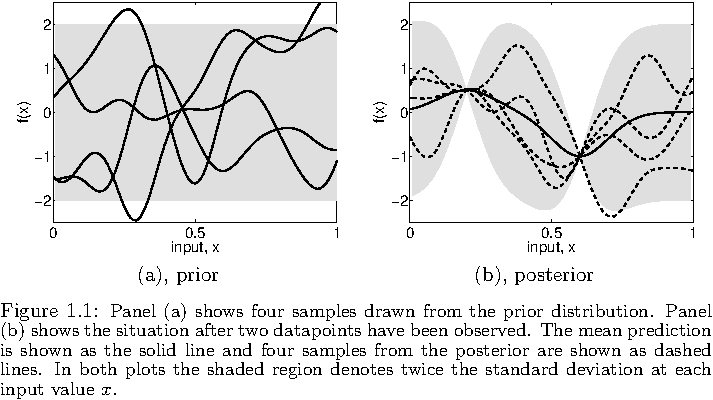
\includegraphics[width=\textwidth]{samples.pdf}
\end{frame}

\begin{frame} \frametitle{GP: Weight space view}
\begin{itemize}
  \item Model a linear function with some Gaussian noise:
  \begin{equation}
    f(\vec{x}) = \vec{x}\T\vec{w}, \quad
    y = f(\vec{x}) + \epsilon, \quad
    \epsilon \sim \N{0,\sigma_n^2}
  \end{equation}
  \item This implies the likelihood, the probability density of the
    observations given the parameters:
  \begin{equation}
    p(\vec{y}|X,\vec{w}) = \N{X\T\vec{w},\,\sigma_n^2I}
  \end{equation}
  \item Putting a prior on $\vec{w}$ and using Bayes' theorem yields a
    posterior distribution:
  \begin{equation}
    \vec{w} \sim \N{\vec{0},\Sigma_p}
    \quad\Rightarrow\quad
    p(\vec{w}|X,\vec{y}) = \N{\sigma_n^{-2}A^{-1}X\vec{y},\,A^{-1}},
  \end{equation}
    where $A = \sigma_n^{-2}XX\T + \Sigma_p^{-1}$.
  \item This is like doing a linear fit using infinite-dimensional function
    basis. Weight is synonymous to fit parameter in this language.
\end{itemize}
% Kernel trick would be mentioned here
\end{frame}

\begin{frame} \frametitle{Relation to Neural Networks}
\begin{itemize}
  \item Bayesian neural networks because Gaussian processes in the limit of the
    number of hidden nodes approaching infinity.
  \begin{itemize}
    \item Neal, R.M. Bayesian Learning for Neural Networks.\\
      Springer Verlag, 1996. ISBN 0387947248.
  \end{itemize}
\end{itemize}
\end{frame}

\newcommand{\plot}[2][0.36]{%
  \includegraphics[width=#1\textwidth]{gp/{#2}.pdf}
}

\begin{frame} \frametitle{Squared Exponential Kernel}
% \vspace{-1mm}
\textbf{Synonims}: Radial Basis Function, Gaussian, Exponentiated Quadratic
\begin{equation}
  k(x,x') = \exp\left(-\frac{\left|x-x'\right|^2}{2\ell^2}\right)
\end{equation}
  \vspace{-3mm}
\begin{itemize}
  \item The de-facto default kernel.
  \item Produces infinitely differentiable functions.
  \item $\ell$ - lengthscale. Determines the scale of function's features.
    Generally, cannot extrapolate farther than distance $\ell$ from the data.
  \item Stationary: depends only on $x-x'$.
  \item Isotropic: depends only on $|x-x'|$.
\end{itemize}
\vspace{-2mm}
\begin{center}
  \plot[0.5]{js_se_0_1_1.5}
\end{center}
\end{frame}

\begin{frame} \frametitle{Noise and signal variances}
\vspace{-2mm}
\begin{itemize}
  \item Typically, two extra parameters are added to the kernel model.
  \item $\sigma_s^2$ - signal variance.
    This is a multiplicative factor attached to every additive term in a
    kernel.
    Determines the average distance of the function away from the mean.
  \item $\sigma_n^2$ - noise variance.
    This is added to the diagonal elements of the kernel, and provides a
    measure of the observation's uncertainty.
  \item With both terms introduced, the SE kernel looks like this
\end{itemize}
\begin{equation}
  k(x,x') = \sigma_s^2 \exp\left(-\frac{\left|x-x'\right|^2}{2\ell^2}\right)
          + \sigma_n^2 \delta_{xx'}
\end{equation}
\vspace{-2.5mm}
\begin{itemize}
  \item $\sigma_n^2$ can be different for every point, e.g. Poisson
    uncertainties for a histogram.
\end{itemize}
\vspace{-4mm}
\begin{changemargin}{-4.3mm}{0mm}
\plot{rw_se_0.1_1_1}
\plot{rw_se_5e-05_1.08_0.3}
\plot{rw_se_0.89_1.16_3}
\end{changemargin}
\end{frame}

\begin{frame} \frametitle{Rational Quadratic Kernel}
\begin{equation}
  k(x,x') = \left( 1 + \frac{\left|x-x'\right|^2}{2\alpha\ell^2} \right)^{-\alpha}
\end{equation}
\begin{itemize}
  \item Equivalent to a series of SE kernels with different length scales.
  \item $\alpha$ - determines the relative weighting of large-scale and
    small-scale variations.
  \item RQ $\rightarrow$ SE as $\alpha\rightarrow\infty$.
\end{itemize}
\begin{center}
  \plot[0.5]{js_rq_0_1_1.5_2}
\end{center}
\end{frame}

\begin{frame} \frametitle{Periodic Kernel}
\begin{equation}
  k(x,x') = \exp\left(-\frac{2}{\ell^2}\sin^2\left[\frac{\pi|x - x'|}{\lambda}\right]\right)
\end{equation}
\begin{itemize}
  \item Allows to model functions with exact periodicity.
\end{itemize}
\end{frame}

\begin{frame} \frametitle{Mat\'ern Kernel}
\vspace{-3mm}
\begin{equation}
  k(d) = \frac{2^{1-\nu}}{\Gamma(\nu)}\Bigg(\sqrt{2\nu}\,\frac{r}{\rho}\Bigg)^\nu
    K_\nu\Bigg(\sqrt{2\nu}\,\frac{r}{\rho}\Bigg)
\end{equation}
\vspace{-3mm}
\begin{itemize}
  \item $r = |x-x'|$
  \item $\Gamma$ - gamma function
  \item $K_\nu$ - modified Bessel function of the second kind
  \item $\rho$ and $\nu$ are non-negative parameters.
  \item Yields sample paths that are $\lceil\nu\rceil - 1$ times differentiable.
\end{itemize}
\begin{center}
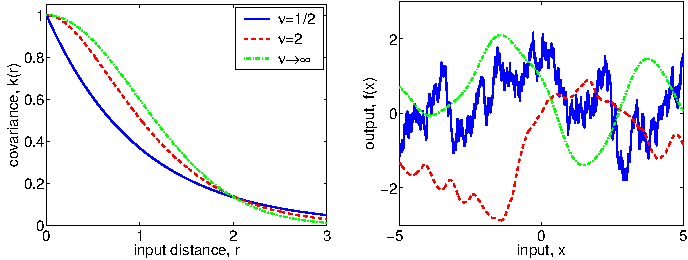
\includegraphics[width=0.8\textwidth]{matern}
\end{center}
\PlaceText{0.24}{0.91}{{\small kernel functions}}
\PlaceText{0.61}{0.91}{{\small sampled functions}}
\PlaceText{0.88}{0.81}{{\color{gray}\scriptsize Figure from}}
\PlaceText{0.88}{0.84}{{\color{gray}\scriptsize Rasmussen}}
\PlaceText{0.88}{0.87}{{\color{gray}\scriptsize \& Williams}}
\end{frame}

\begin{frame} \frametitle{Kernel Composition}
\begin{itemize}
  \item Allows to better capture features on different scales
  \item Multiplication: AND operation
  \item Addition: OR operation
  \item Example: Locally periodic kernel
\end{itemize}
\begin{equation}
  k(x,x') =
  \exp\left(-\frac{2}{\ell_1^2}\sin^2\left[\frac{\pi|x - x'|}{\lambda}\right]\right)
  \exp\left(-\frac{\left|x-x'\right|^2}{2\ell_2^2}\right)
\end{equation}
\end{frame}

\begin{frame} \frametitle{Optimization of Kernel Parameters}
\begin{itemize}
  \item Need to maximize $p(\theta|x,y)$.
  \item By the Bayes' theorem, this is the same as maximizing $p(y|x,\theta)$.
  \item This is the prior.
\end{itemize}
\begin{equation}
  \vec{y} \sim \N{\vec{0},K}
\end{equation}
\begin{itemize}
  \item Therefore, optimal parameters are given my maximizing log prior
    likelihood:
\end{itemize}
\begin{equation}
  \log p(y) = - \tfrac{1}{2}\vec{y}\T K^{-1}\vec{y}
              - \tfrac{1}{2}\log|K| - \tfrac{n}{2}\log 2\pi
\end{equation}
\begin{itemize}
  \item Knowledge of the specific problem may dictate more appropriate kernel
    parameters.
  \begin{itemize}
    \item For example, noise variance may be known.
    \item Length scale may have a physical meaning.
  \end{itemize}
\end{itemize}
\end{frame}

% \begin{frame} \frametitle{GP for Classification}
% \end{frame}

\newcommand{\R}[2]{\item #1 \\ {\scriptsize\url{#2}}}
\newcommand{\arxiv}[1]{arXiv:\href{https://arxiv.org/abs/#1}{#1}}

\begin{frame} \frametitle{References}
\begin{itemize}
  \R{Rasmussen \& Williams (the cannonical textbook)}
    {http://www.gaussianprocess.org/gpml/chapters/}
  \R{Mark Ebden {\small(simpler introduction than R\&W)}}
    {https://arxiv.org/abs/1505.02965}
  \R{Katherine Bailey {\small(simple python\,\plus\,numpy code)}}
    {http://katbailey.github.io/post/gaussian-processes-for-dummies/}
  \R{CS229 Stanford Notes (Chuong Do)}
    {http://cs229.stanford.edu/section/cs229-gaussian_processes.pdf}
  \R{Kernel Cookbook (David Duvenaud)}
    {https://www.cs.toronto.edu/~duvenaud/cookbook/}
  \R{Rob Fletcher's slides (ATLAS internal)}
    {https://indico.cern.ch/event/744257/contributions/3077617/attachments/1688169/2715519/GP_Fletcher.pdf}
  \item Some interesting papers:
  \begin{itemize}
    \item \arxiv{1709.05681} (Modeling smooth backgrounds)
    \item \arxiv{1302.4245} (Spectral mixture kernel)
  \end{itemize}
\end{itemize}
\end{frame}

